% \documentclass{article}
% \usepackage{graphicx} % Required for inserting images
% \ libs 
\documentclass{article}
\usepackage{graphicx}
\usepackage[utf8]{inputenc}
\usepackage[brazil]{babel} 
\usepackage[top=2cm, bottom=2cm, left=3cm, right=2cm]{geometry}
\usepackage{circuitikz}
\usepackage{siunitx}
\usepackage{multirow}
\usepackage[font=footnotesize,bf]{caption} 
\captionsetup{font={footnotesize}}
% Espaçamento 1.5
\usepackage{setspace}
\setstretch{1.5}
\usepackage{gensymb}
% Pacote para equações num quadrado
\usepackage{amsmath}
\usepackage{tikz}
\usepackage{mathdots}
\usepackage{yhmath}
\usepackage{cancel}
\usepackage{color}
\usepackage{array}
\usepackage{multirow}
\usepackage{amssymb}
\usepackage{gensymb}
\usepackage{tabularx}
\usepackage{booktabs}
\usetikzlibrary{fadings}
\usepackage{float} 
\usepackage{blindtext}
\usepackage{hyperref}
\usepackage{textcomp, gensymb}
% Pacote Subfigure
\usepackage{subfigure}
\usepackage{longtable}
% Cabeçalho e Rodapé
 \usepackage{fancyhdr}
\usepackage[alf]{abntex2cite}
\usepackage{enumerate}

% \usepackage{minted}
\usepackage{algorithm2e}
% Configuração de palavras-chave para português

% Pacotes e configurações para inserir códigos
\usepackage{listings}
\lstdefinelanguage{VHDL}{
  morekeywords=[1]{library,use,entity,port,architecture,begin,end,is,signal,when,else,with,select,not,and,or,xor,in,out,std_logic,std_logic_vector},
  sensitive=true,
  morecomment=[l]--,
  morestring=[b]"
}

\lstset{
  language=VHDL,
  basicstyle=\ttfamily\footnotesize,
  keywordstyle=\color{blue}\bfseries,
  commentstyle=\color{gray},
  stringstyle=\color{orange},
  numbers=left,
  numberstyle=\tiny,
  stepnumber=1,
  numbersep=8pt,
  tabsize=2,
  showstringspaces=false,
  breaklines=true,
  breakatwhitespace=false,
  frame=single,
  captionpos=b
}

\usepackage{xcolor}

% \title{Artigo Problema NP-Completo}
% \author{Alberto Magno, Josué Nogueira, Leonardo Avelar}
% \date{April 2025}

\begin{document}

\pagestyle{fancy} %estilo fancy
\lhead{\rightmark} % esquerda do cabeçalho
\chead{} %centro do cabeçalho
\rhead{\leftmark} % direita do cabeçalho
\lfoot{ALU VHDL} %esquerda do rodapé
 
\cfoot{\thepage} %centro do rodapé
\rfoot{Sistemas Reconfiguráveis} %direita do rodapé
\renewcommand{\footrulewidth}{1pt}

% \begin{titlepage}

%     \newcommand{\HRule}{\rule{\linewidth}{0.0mm}} % Defines a new command for the horizontal lines, change thickness here
    
%     \center % Center everything on the page
     
%     %----------------------------------------------------------------------------------------
%     %	HEADING SECTIONS
%     %----------------------------------------------------------------------------------------
    
%     \textsc{Pontifícia Universidade Católica de Minas Gerais}\\[0.5cm] % Name of your university/college
%     \vskip-.5cm
%     \textsc{Instituto de Ciências Exatas e Computação}\\[0.5cm] % Name of your university/college
%     \vskip-.5cm
%     \textsc{Engenharia de Computação}\\[0.5cm] % Major heading such as course name
%     \vskip-.5cm
    
    
%     %----------------------------------------------------------------------------------------
%     %	TITLE SECTION
%     %----------------------------------------------------------------------------------------
%     \vskip3cm
%     \HRule \\[0.4cm]
%     {\huge \bfseries PRIMEIRO TRABALHO DE SISTEMAS RECONFIGURÁVEIS}\\[0.4cm] % Title of your document
%     \HRule \\[1cm]
     
%     %----------------------------------------------------------------------------------------
%     %	AUTHOR SECTION
%     %----------------------------------------------------------------------------------------
%     \vskip1cm
%     \begin{minipage}{0.8\textwidth}
%     \begin{flushleft} 
%     \textbf{Alunos:}\\
%     \paragraph{}Alberto Magno Machado
%     \paragraph{}Ana Luiza Diniz Santos
%     \paragraph{}Pablo Marcelino Las-Cazas
    
%     \vskip1cm
%     \textbf{Professor:} \\
%     \paragraph{}{Francisco Garcia} 
%     \end{flushleft}
%     \end{minipage}
    
%     \end{titlepage}
\begin{titlepage}
    \centering

    % Logo da PUC Minas
    
\includegraphics[width=4cm]{images/logo_pucminas.png}\\[1cm]

    {\large\textbf{PONTIFÍCIA UNIVERSIDADE CATÓLICA DE MINAS GERAIS}}\\[0.3cm]
    {\large\textbf{Instituto de Ciências Exatas e Informática}}\\[0.3cm]
    {\large\textbf{Curso de Engenharia de Computação}}\\[5cm]

    {\Large\bfseries UNIDADE LÓGICA E ARITMÉTICA VHDL}\\[5cm]

    \begin{flushright}
        \textbf{Alunos:}\\
        Alberto Magno Machado\\
        Ana Luiza Diniz Santos\\
        Pablo Marcelino Las-Cazas
    \end{flushright}

    \vfill

    \textbf{Belo Horizonte}\\
    \textbf{Abril de 2025}
\end{titlepage}


% \begin{titlepage}
%     \centering
%     {\large\textbf{PONTIFÍCIA UNIVERSIDADE CATÓLICA DE MINAS GERAIS}}\\[0.5cm]
%     {\large\textbf{Instituto de Ciências Exatas e Computação}}\\[0.2cm]
%     {\large\textbf{Engenharia de Computação}}\\[3cm]

%     {\Large\bfseries UNIDADE LÓGICA E ARITMÉTICA VHDL}\\[3cm]

%     \textbf{Alunos:}\\
%     Alberto Magno Machado\\
%     Ana Luiza Diniz Santos\\
%     Pablo Marcelino Las-Cazas\\[2cm]

%     \textbf{Professor:}\\
%     Francisco Garcia\\[3.5cm]

%     \vfill

%     Belo Horizonte\\
%     Abril de 2025
% \end{titlepage}

\begin{titlepage}
    \centering
    {\large\textbf{PONTIFÍCIA UNIVERSIDADE CATÓLICA DE MINAS GERAIS}}\\[0.5cm]
    {\large\textbf{Instituto de Ciências Exatas e Informática}}\\[0.2cm]
    {\large\textbf{Curso de Engenharia de Computação}}\\[6cm]

    {\Large\bfseries UNIDADE LÓGICA E ARITMÉTICA}\\[3cm]

    \begin{flushright}
    Trabalho desenvolvido para a matéria de 
    
    Sistemas Reconfiguráveis do curso de 
    
    Engenharia de Computação da PUC Minas.\\[0.8cm]

    Professor: Francisco Garcia
    \end{flushright}

    \vfill
    \textbf{Belo Horizonte}\\
    Abril de 2025
\end{titlepage}



\tableofcontents
\pagebreak
\listoffigures
\pagebreak
\listoftables
\pagebreak

\section{Introdução}

A arquitetura de sistemas digitais modernos exige componentes versáteis e eficientes para o processamento de dados. Dentre esses componentes, a Unidade Lógica e Aritmética (ALU – Arithmetic and Logic Unit) desempenha um papel central na execução de operações fundamentais como somas, subtrações, operações lógicas e manipulações de bits.

Este trabalho tem como objetivo o desenvolvimento de uma ALU de 8 bits utilizando a linguagem de descrição de hardware VHDL, respeitando os princípios de design digital combinacional. O projeto foi implementado no ambiente Quartus II 9.1sp2, sendo exclusivamente composto por código concorrente, sem a utilização de elementos sequenciais como flip-flops ou latches. A ALU implementada é capaz de realizar 16 operações distintas, incluindo operações aritméticas com e sem carry, operações lógicas bit a bit, rotações e deslocamentos.

O relatório está organizado da seguinte forma: na seção 2 são apresentados os requisitos do projeto; a seção 3 descreve o desenvolvimento da ALU, incluindo decisões de projeto e trechos de código relevantes; a seção 4 detalha os testes realizados e os resultados obtidos; por fim, a seção 5 apresenta as considerações finais.
\pagebreak
\section{Requisitos do Projeto}

O presente trabalho tem como finalidade o desenvolvimento de uma Unidade Lógica e Aritmética (ALU) descrita em VHDL, operando com palavras de 8 bits e implementada de forma totalmente combinacional. O projeto deve ser implementado e simulado utilizando exclusivamente a versão 9.1sp2 do software Quartus II.

A seguir, são apresentados os requisitos funcionais e técnicos que a ALU deve atender.

\subsection{Requisitos Funcionais}

A ALU deve ser capaz de realizar 16 operações distintas, conforme o valor de entrada de seleção de operação (\texttt{op\_sel[3..0]}), agrupadas em:

\subsubsection*{Operações Aritméticas}

\begin{table}[H]
\centering
\begin{tabular}{|c|c|l|}
\hline
\textbf{op\_sel} & \textbf{Mnemônico} & \textbf{Descrição} \\ \hline
0000 & ADD  & Soma sem carry-in: $r\_out = a + b$ \\ \hline
0001 & ADDC & Soma com carry-in: $r\_out = a + b + c\_in$ \\ \hline
0010 & SUB  & Subtração sem carry-in: $r\_out = a - b$ \\ \hline
0011 & SUBC & Subtração com carry-in: $r\_out = a - b - c\_in$ \\ \hline
\end{tabular}
\caption{Operações aritméticas}
\end{table}

\subsubsection*{Operações Lógicas}

\begin{table}[H]
\centering
\begin{tabular}{|c|c|l|}
\hline
\textbf{op\_sel} & \textbf{Mnemônico} & \textbf{Descrição} \\ \hline
0100 & AND  & AND lógico bit a bit: $r\_out = a \land b$ \\ \hline
0101 & OR   & OR lógico bit a bit: $r\_out = a \lor b$ \\ \hline
0110 & XOR  & XOR lógico bit a bit: $r\_out = a \oplus b$ \\ \hline
0111 & NOT  & Complemento bit a bit: $r\_out = \sim a$ \\ \hline
\end{tabular}
\caption{Operações lógicas}
\end{table}

\subsubsection*{Rotações e Deslocamentos}

\begin{table}[H]
\centering
\begin{tabular}{|c|c|l|}
\hline
\textbf{op\_sel} & \textbf{Mnemônico} & \textbf{Descrição} \\ \hline
1000 & RL   & Rotação à esquerda: $r\_out = a[6..0], a[7]$ \\ \hline
1001 & RR   & Rotação à direita: $r\_out = a[0], a[7..1]$ \\ \hline
1010 & RLC  & Rotação à esquerda via carry: $r\_out = a[6..0], c\_in$ \\ \hline
1011 & RRC  & Rotação à direita via carry: $r\_out = c\_in, a[7..1]$ \\ \hline
1100 & SLL  & Deslocamento lógico à esquerda: $r\_out = a[6..0], 0$ \\ \hline
1101 & SRL  & Deslocamento lógico à direita: $r\_out = 0, a[7..1]$ \\ \hline
1110 & SRA  & Deslocamento aritmético à direita: $r\_out = a[7], a[7..1]$ \\ \hline
\end{tabular}
\caption{Rotações e deslocamentos}
\end{table}

\subsubsection*{Bypass}

\begin{table}[H]
\centering
\begin{tabular}{|c|c|l|}
\hline
\textbf{op\_sel} & \textbf{Mnemônico} & \textbf{Descrição} \\ \hline
1111 & PASS\_B & Passa o valor de \texttt{b\_in} diretamente: $r\_out = b$ \\ \hline
\end{tabular}
\caption{Operação de bypass}
\end{table}

\pagebreak
\section{Desenvolvimento}

A ALU foi implementada utilizando a linguagem VHDL, respeitando a estrutura combinacional exigida no projeto, sem o uso de elementos sequenciais como \textit{flip-flops} ou \textit{latches}.

\subsection{Implementação VHDL}

A seguir, apresenta-se a declaração da entidade \texttt{alu}, incluindo as portas de entrada e saída:

\begin{figure}[H]
\centering
\lstinputlisting[language=VHDL, firstline=1, lastline=19, caption={Declaração da entidade \texttt{alu}}, label={lst:alu-entity}]{code/alu.vhd}
\end{figure}

A seguir, são apresentados os sinais internos utilizados na arquitetura:

\begin{figure}[H]
\centering
\lstinputlisting[language=VHDL, firstline=21, lastline=24, caption={Declaração dos sinais internos}, label={lst:alu-signals}]{code/alu.vhd}
\end{figure}

A implementação das operações de soma e subtração com e sem carry pode ser vista abaixo:

\begin{figure}[H]
\centering
\lstinputlisting[language=VHDL, firstline=26, lastline=36, caption={Cálculo de soma e subtração}, label={lst:alu-add-sub}]{code/alu.vhd}
\end{figure}

As 16 operações são selecionadas por meio da diretiva \texttt{with...select}, conforme segue:

\begin{figure}[H]
\centering
\lstinputlisting[language=VHDL, firstline=39, lastline=58, caption={Bloco de seleção de operações da ALU}, label={lst:alu-opselect}]{code/alu.vhd}
\end{figure}    

A lógica de atribuição do sinal \texttt{c\_out} considera o tipo de operação realizada:

\begin{figure}[H]
\centering
\lstinputlisting[language=VHDL, firstline=60, lastline=66, caption={Atribuição de \texttt{c\_out}}, label={lst:alu-cout}]{code/alu.vhd}
\end{figure}

O sinal \texttt{z\_out} é ativado quando o resultado da operação é igual a zero:

\begin{figure}[H]
\centering
\lstinputlisting[language=VHDL, firstline=68, lastline=69, caption={Atribuição de \texttt{z\_out}}, label={lst:alu-zout}]{code/alu.vhd}
\end{figure}

A lógica de \texttt{v\_out} detecta overflow nas operações aritméticas:

\begin{figure}[H]
\centering
\lstinputlisting[language=VHDL, firstline=71, lastline=79, caption={Atribuição de \texttt{v\_out}}, label={lst:alu-vout}]{code/alu.vhd}
\end{figure}

A saída principal da ALU é atribuída com o valor de \texttt{temp\_r}:

\begin{figure}[H]
\centering
\lstinputlisting[language=VHDL, firstline=81, lastline=83, caption={Atribuição final da saída \texttt{r\_out}}, label={lst:alu-rout}]{code/alu.vhd}
\end{figure}

\subsection{Organização dos Arquivos do Projeto}

O projeto foi salvo no diretório \texttt{E1\_ALU/ALU}, contendo os seguintes arquivos principais:

\begin{itemize}
  \item \textbf{alu.vhd}: código-fonte VHDL da ALU, com estrutura combinacional.
  
  \item \textbf{alu.vwf}: arquivo de forma de onda (Waveform File), utilizado para simulação no Quartus II.
  
  \item \textbf{Relatórios de compilação}: arquivos com extensão \texttt{.rpt}, \texttt{.summary}, \texttt{.sof}, \texttt{.pof}, entre outros, gerados automaticamente pelo ambiente de desenvolvimento Quartus II durante a síntese e análise do projeto.
  
  \item \textbf{alu.sim.rpt}: relatório contendo os resultados das simulações funcionais realizadas sobre o circuito.
  
  \item \textbf{alu.done}: arquivo que indica a compilação bem-sucedida do projeto.
\end{itemize}


    

\pagebreak
\section{Testes e Resultados}

Após a implementação da ALU, foram realizados testes para cada uma das 16 operações especificadas. As simulações foram feitas utilizando o editor de formas de onda (VWF) do Quartus II, com diferentes valores de entrada para os sinais \texttt{a\_in}, \texttt{b\_in}, \texttt{c\_in} e \texttt{op\_sel}. Cada teste resultou em uma imagem capturada da simulação, localizada na pasta \texttt{Testes/} do projeto.

A seguir, são apresentados os resultados obtidos em cada operação, com a respectiva análise.

\subsection{Operações Aritméticas}

\begin{figure}[H]
\centering
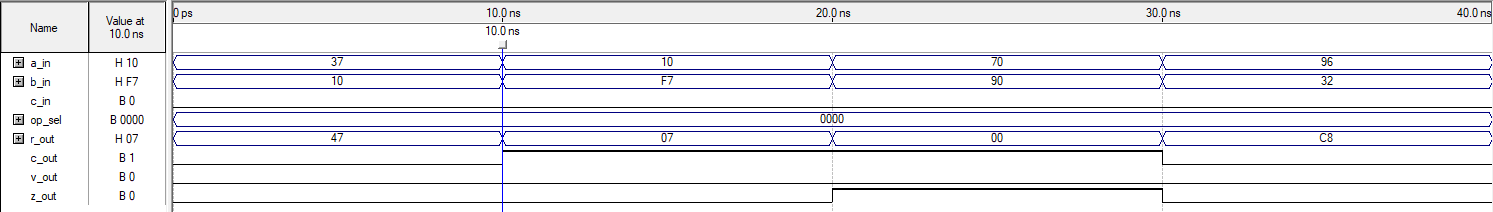
\includegraphics[width=\textwidth]{images/alu_0000.png}
\caption{Operação ADD (\texttt{op\_sel = 0000}): Soma sem carry-in}
\end{figure}

Nesta simulação, observa-se que o valor de \texttt{r\_out} corresponde corretamente à soma de \texttt{a\_in} e \texttt{b\_in}. O sinal \texttt{c\_out} indica a ocorrência (ou não) de carry, e \texttt{v\_out} sinaliza overflow quando aplicável.

\begin{figure}[H]
\centering
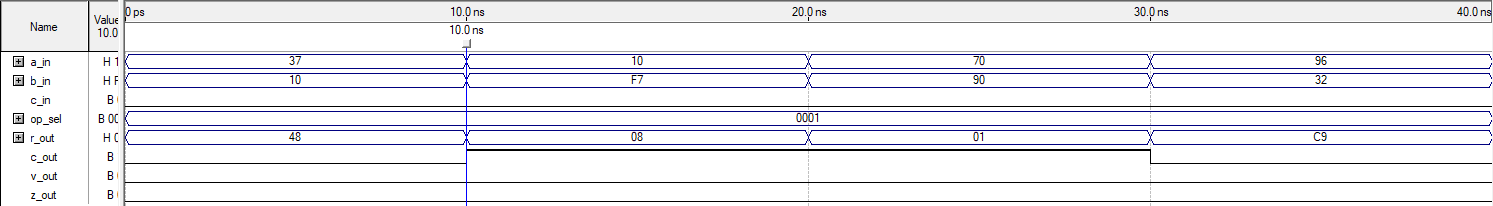
\includegraphics[width=\textwidth]{images/alu_0001.png}
\caption{Operação ADDC (\texttt{op\_sel = 0001}): Soma com carry-in}
\end{figure}

Neste caso, o bit de carry-in (\texttt{c\_in}) é adicionado ao resultado, afetando tanto o valor de saída quanto o \texttt{c\_out} final.

\begin{figure}[H]
\centering
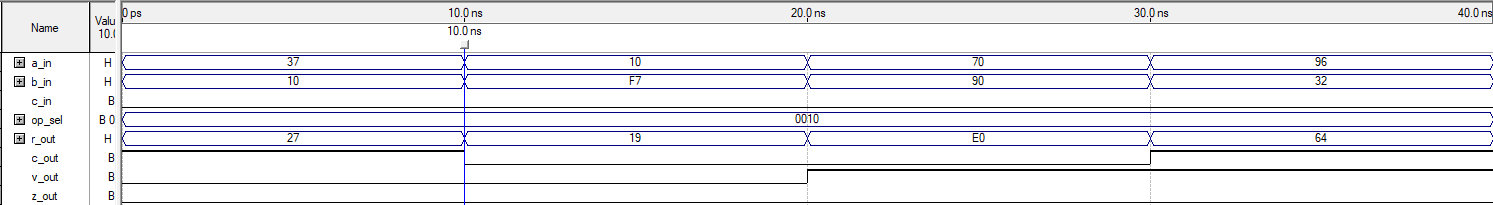
\includegraphics[width=\textwidth]{images/alu_0010.png}
\caption{Operação SUB (\texttt{op\_sel = 0010}): Subtração sem carry-in}
\end{figure}

A subtração simples de \texttt{a\_in} menos \texttt{b\_in} é realizada, e o \texttt{c\_out} representa o borrow.

\begin{figure}[H]
\centering
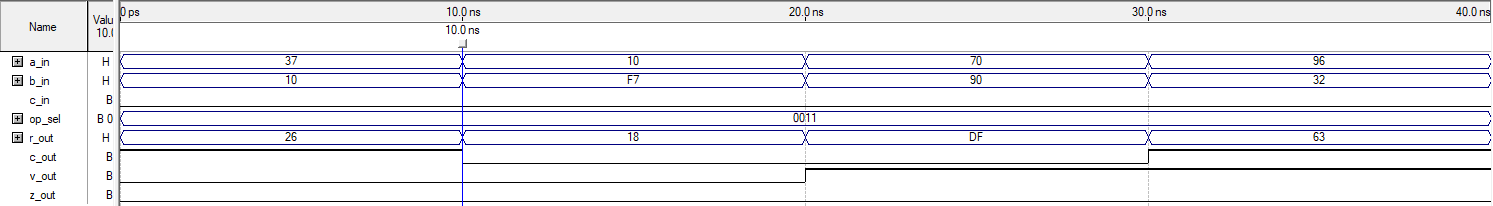
\includegraphics[width=\textwidth]{images/alu_0011.png}
\caption{Operação SUBC (\texttt{op\_sel = 0011}): Subtração com carry-in}
\end{figure}

A subtração considera o carry-in como um decrementador adicional, afetando o resultado final e os sinais auxiliares.

\subsection{Operações Lógicas}

\begin{figure}[H]
\centering
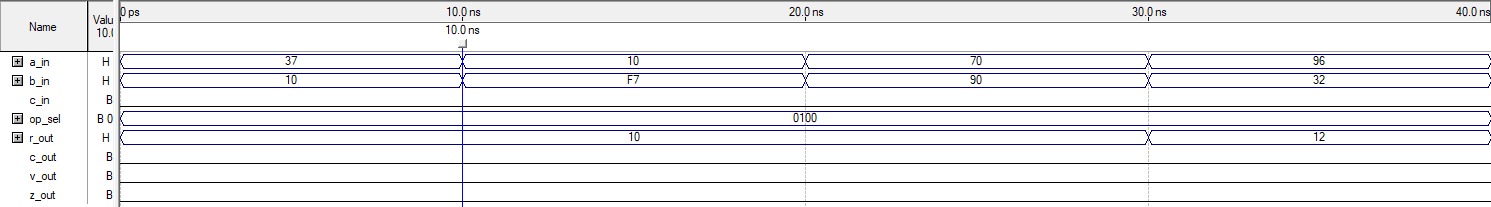
\includegraphics[width=\textwidth]{images/alu_0100.png}
\caption{Operação AND (\texttt{op\_sel = 0100})}
\end{figure}

A saída corresponde ao resultado do AND bit a bit entre os operandos \texttt{a\_in} e \texttt{b\_in}. O sinal \texttt{z\_out} indica se o resultado foi nulo.

\begin{figure}[H]
\centering
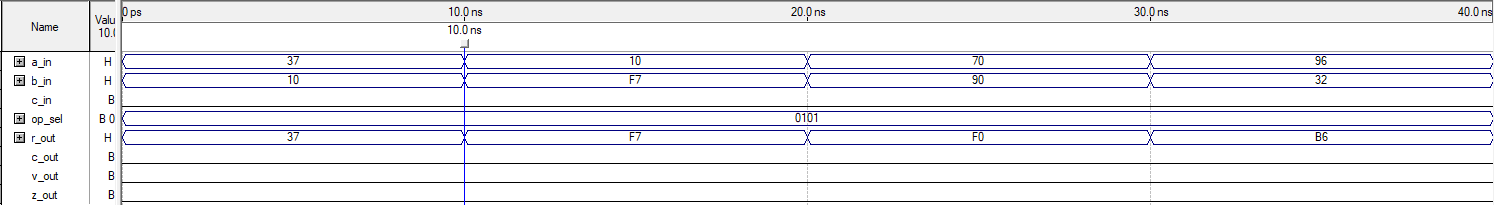
\includegraphics[width=\textwidth]{images/alu_0101.png}
\caption{Operação OR (\texttt{op\_sel = 0101})}
\end{figure}

Operação OR bit a bit entre os dois operandos, útil para ativar bits em paralelo.

\begin{figure}[H]
\centering
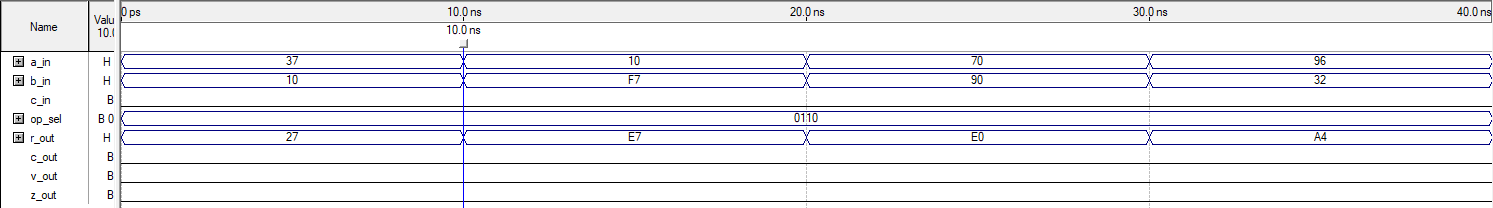
\includegraphics[width=\textwidth]{images/alu_0110.png}
\caption{Operação XOR (\texttt{op\_sel = 0110})}
\end{figure}

Realiza o XOR bit a bit, com o sinal de zero sendo ativado se todos os bits da saída forem '0'.

\begin{figure}[H]
\centering
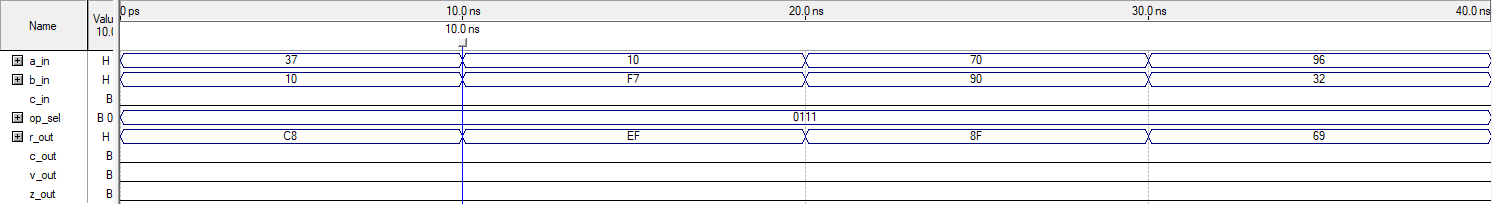
\includegraphics[width=\textwidth]{images/alu_0111.png}
\caption{Operação NOT (\texttt{op\_sel = 0111})}
\end{figure}

Complementa todos os bits de \texttt{a\_in}, ignorando \texttt{b\_in} e \texttt{c\_in}.

\subsection{Rotações e Deslocamentos}

\begin{figure}[H]
\centering
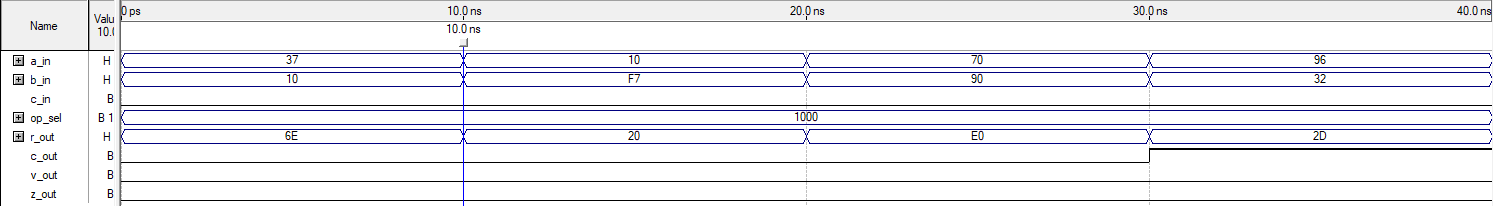
\includegraphics[width=\textwidth]{images/alu_1000.png}
\caption{Operação RL (\texttt{op\_sel = 1000}): Rotação para a esquerda}
\end{figure}

Rotaciona os bits de \texttt{a\_in} para a esquerda, com o bit mais significativo indo para a posição menos significativa.

\begin{figure}[H]
\centering
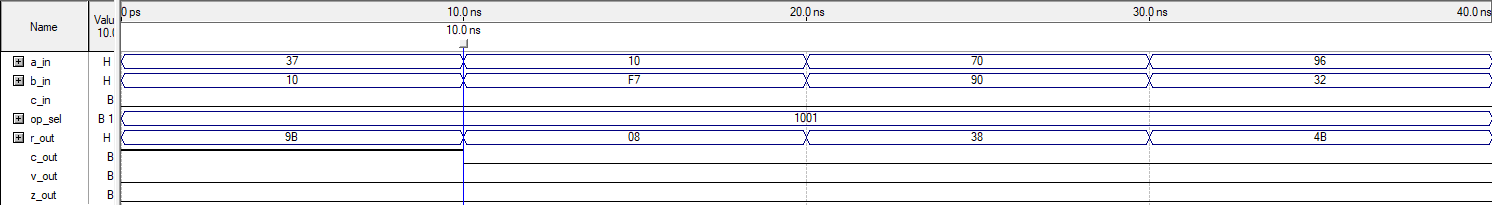
\includegraphics[width=\textwidth]{images/alu_1001.png}
\caption{Operação RR (\texttt{op\_sel = 1001}): Rotação para a direita}
\end{figure}

Rotação simples para a direita, levando o LSB para o MSB.

\begin{figure}[H]
\centering
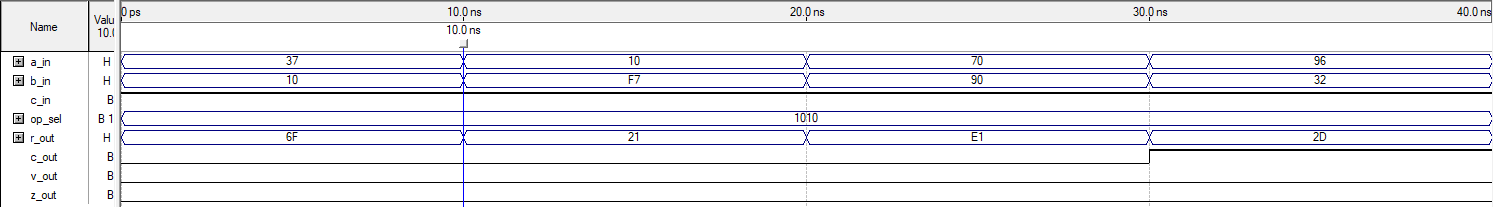
\includegraphics[width=\textwidth]{images/alu_1010.png}
\caption{Operação RLC (\texttt{op\_sel = 1010}): Rotação à esquerda via carry}
\end{figure}

Aqui, o bit de carry-in é inserido como LSB, e o MSB de \texttt{a\_in} torna-se o \texttt{c\_out}.

\begin{figure}[H]
\centering
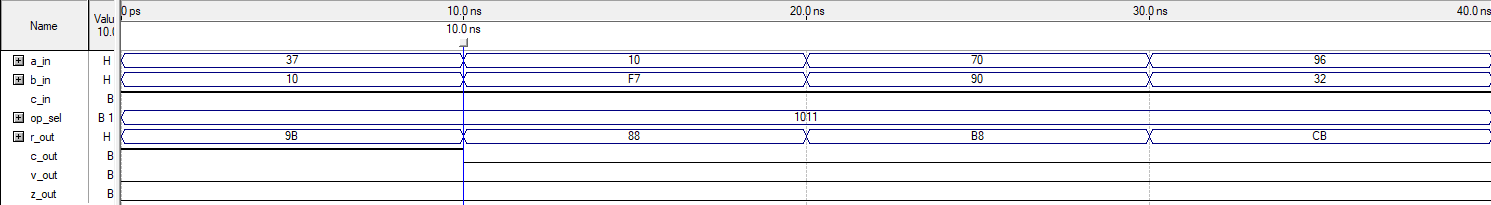
\includegraphics[width=\textwidth]{images/alu_1011.png}
\caption{Operação RRC (\texttt{op\_sel = 1011}): Rotação à direita via carry}
\end{figure}

Similar à RLC, mas rotacionando para a direita. O carry-in ocupa o MSB, e o LSB vira \texttt{c\_out}.

\begin{figure}[H]
\centering
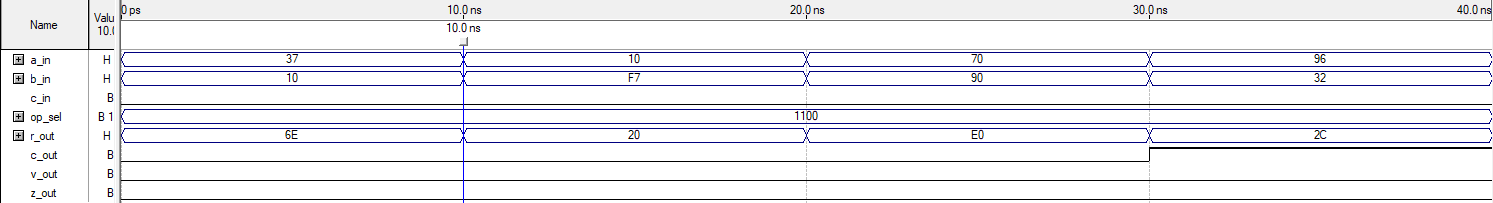
\includegraphics[width=\textwidth]{images/alu_1100.png}
\caption{Operação SLL (\texttt{op\_sel = 1100}): Deslocamento lógico à esquerda}
\end{figure}

Desloca os bits à esquerda e insere zero no LSB.

\begin{figure}[H]
\centering
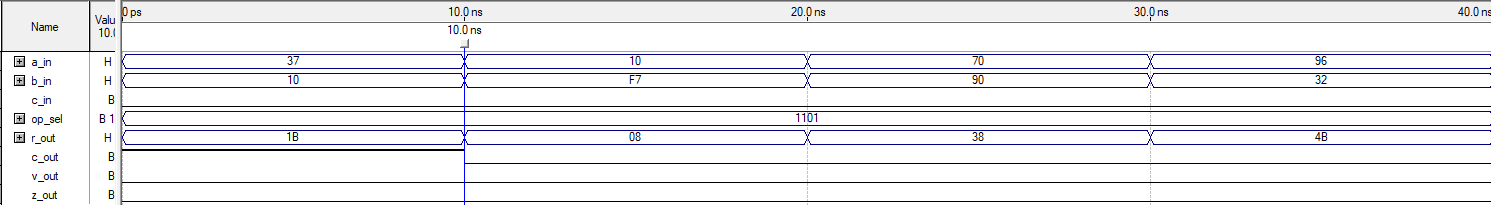
\includegraphics[width=\textwidth]{images/alu_1101.png}
\caption{Operação SRL (\texttt{op\_sel = 1101}): Deslocamento lógico à direita}
\end{figure}

Desloca os bits à direita, preenchendo o MSB com zero.

\begin{figure}[H]
\centering
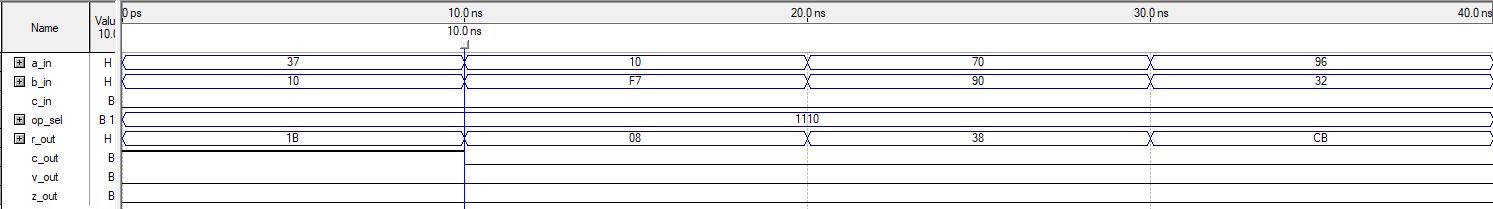
\includegraphics[width=\textwidth]{images/alu_1110.png}
\caption{Operação SRA (\texttt{op\_sel = 1110}): Deslocamento aritmético à direita}
\end{figure}

Mantém o bit de sinal (MSB) ao deslocar bits à direita.

\subsection{Bypass}

\begin{figure}[H]
\centering
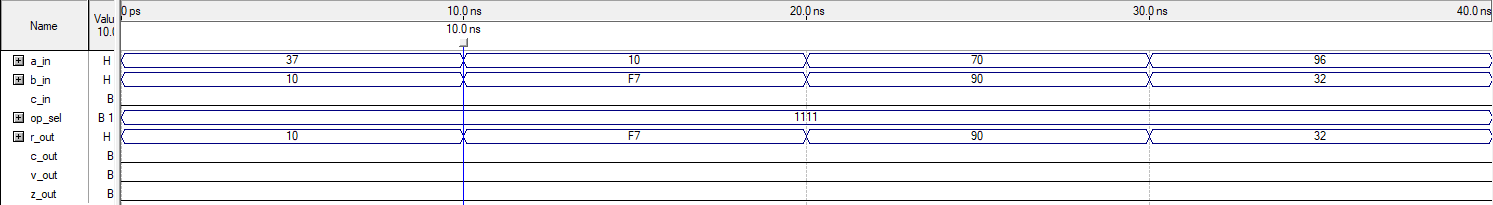
\includegraphics[width=\textwidth]{images/alu_1111.png}
\caption{Operação PASS\_B (\texttt{op\_sel = 1111}): Passagem direta de \texttt{b\_in}}
\end{figure}

Nesta operação, o valor de \texttt{b\_in} é passado diretamente para a saída \texttt{r\_out}, ignorando \texttt{a\_in} e \texttt{c\_in}.
\pagebreak
\section{Conclusão}

O desenvolvimento de uma Unidade Lógica e Aritmética (ALU) de 8 bits utilizando a linguagem VHDL permitiu consolidar conhecimentos teóricos e práticos relacionados à lógica digital, à modelagem de hardware e ao uso do ambiente de desenvolvimento Quartus II.

A implementação foi conduzida de forma estruturada, respeitando os requisitos propostos, com a construção de um circuito totalmente combinacional e a aplicação de técnicas de codificação concorrente. A ALU resultante foi capaz de executar corretamente as 16 operações especificadas, incluindo funções aritméticas, lógicas, rotações e deslocamentos, além de sinalizar adequadamente os estados de carry, zero e overflow.

As simulações realizadas confirmaram a conformidade do comportamento funcional do projeto com as especificações fornecidas. O uso de arquivos de forma de onda (\texttt{.vwf}) e os relatórios de simulação evidenciaram que todas as operações foram validadas com sucesso.
\pagebreak
\begin{thebibliography}{99}

    \bibitem{blog-payroll}
    Witscad. \textit{Arithmetic Logic Unit Design}. Disponível em: \url{https://witscad.com/course/computer-architecture/chapter/arithmetic-logic-unit-design}.
    
    \bibitem{vhdl-manual}
    Staff. \textit{VHDL References Manual}. Disponível em: \url{https://staff.fysik.su.se/~silver/digsyst/vhdl_ref.pdf}
    
    \bibitem{quartus-manual}
    Intel Corporation. \textit{Quartus II Handbook, Version 9.1sp2}.
\end{thebibliography}
    
\pagebreak

\end{document}
